\chapter{Obsah CD}

Adresáře zdrojových kódů jsou na CD přiloženy ve formě prostých adresářů a zároveň ve formě stejně pojmenovaných archivů {\tt *.tar.gz}. Tyto archivy pro zjednodušení nejsou v~seznamu níže znovu uváděny.

\begin{itemize}
  \item {\tt projekt.pdf} -- Technická zpráva ve formátu PDF
  \item {\tt projekt} -- Zdrojové soubory technické zprávy

  \item {\tt wildfly-8.0.0.Final} -- Živé demo -- instalace WildFly s~nainstalovanými implementovanými rošířeními, použitelná pro předvedení bakalářské práce (použití v příloze \ref{prilohaPouzivani})

  \item {\tt jsm-policy-subsystem} -- Subsystém WildFly implementovaný jako hlavní součást této práce
  \item {\tt jsm-policy-console-hal} -- Rozšíření webové konzole WildFly umožňující správu výše uvedeného rozšíření (popsané v~kapitole \ref{navrhGUI})
  \item {\tt jsm-policy-test} -- Repozitář integračních testů popsaných v~kapitole \ref{testovani}

  \item {\tt jboss-modules} -- Záplata popsaná v~kapitole \ref{upravaZavadeceWildFly} v~odpovídajícím Git repozitáři
\end{itemize}


\chapter{Postup instalace}\label{prilohaInstalace}

Uvedený postup předpokládá operační systém Linux s~nainstalovaným běhovým prostředím Javy. Testován byl na distribuci Ubuntu 13.10 s~běhovým prostředím Javy OpenJDK 7. Pro odzkoušení systému je možné tento postup přeskočit a využít již nainstalovaný systém podle postupu v~příloze \ref{prilohaPouzivani}.

\begin{enumerate}
  \item Připravte standardní instalaci aplikačního serveru WildFly. Doporučenou verzí je 8.0.0.Final. Postup by měl fungovat i pro novější verze.
  
  \item Proveďte instalaci záplaty {\tt jboss-modules}: (Její účel je popsán v~kapitole \ref{zmenaZaBehu})
  \begin{enumerate}
    \item Nakopírujte do zapisovatelného adresáře repozitář {\tt jboss-modules}. Získat jej můžete ze stejně pojmenovaného adresáře na přiloženém CD nebo z~GitHub:
      \newline\url{https://github.com/honza889/jboss-modules}
    \item Proveďte kompilaci za pomoci nástroje Maven -- v~adresáři {\tt jboss-modules} spusťte: {\tt mvn install}
    \item Výsledným archivem ({\tt target/jboss-modules-*-SNAPSHOT.jar}) nahraďte archiv {\tt jboss-modules.jar} v~adresáři WildFly.
    \item Na začátek spouštěcího skriptu, kterým budete WildFly spouštět, (např. {\tt bin/dom ain.sh}) přidejte:
      \begin{lstlisting}
JAVA_OPTS="$JAVA_OPTS -Djboss.modules.policy-refreshable=true"
      \end{lstlisting}
    \item Po dalším startu by již WildFly měl používat dynamická oprávnění. (viz kapitola \ref{staticPerm})
  \end{enumerate}
  
  \item Proveďte instalaci rozšíření WildFly {\tt jsm-policy-subsystem}:
  \begin{enumerate}
    \item Nakopírujte do zapisovatelného adresáře repozitář {\tt jsm-policy-subsystem}. Získat jej můžete opět z~přiloženého CD nebo z~GitHub:
      \newline\url{https://github.com/honza889/jsm-policy-subsystem}
    \item Proveďte kompilaci za pomoci nástroje Maven: {\tt mvn install}
    \item Výsledný adresář {\tt target/module/org} nahrajte do adresáře {\tt modules/system/la\linebreak yers/base/} v~adresáři WildFly.
    \item Spusťe konzolu WildFly, {\tt bin/jboss-cli.sh} a následujícím příkazem nainstalujte a přidejte subsystém. Pro {\bf standalone} režim:
      \begin{lstlisting}
/extension=org.picketbox.jsmpolicy.subsystem:add
/subsystem=jsmpolicy:add
      \end{lstlisting}
      Pro profil {\tt full} v~režimu {\tt domain}:
      \begin{lstlisting}
/extension=org.picketbox.jsmpolicy.subsystem:add
/profile=full/subsystem=jsmpolicy:add
      \end{lstlisting}
    \item Jestliže se oba příkazy zdaří, subsystém {\tt jsmpolicy} byl úspěšně nainstalován a přidán do profilu. (V~příkladu pro {\tt domain} režim do profilu {\tt full}.)
  \end{enumerate}
  
  \item Proveďte instalaci rozšíření webové konzoly WildFly {\tt jsm-policy-console-hal}:
  \begin{enumerate}
    \item Nakopírujte do zapisovatelného adresáře repozitář {\tt jsm-policy-console-hal}. Získat jej můžete z~přiloženého CD nebo z~GitHub:
      \newline\url{https://github.com/honza889/jsm-policy-console-hal}
    \item Proveďte kompilaci za pomoci nástroje Maven: {\tt mvn install}
    \item Výsledný archiv ({\tt build/app/target/jboss-as-console-*-resources.jar}) nahrajte do adresáře {\tt modules/system/layers/base/org/jboss/as/console/main} v~adresáři WildFly.
    \item Upravte soubor {\tt module.xml}, aby atribut {\tt path} elementu {\tt resource-root} odpovídal názvu souboru zkopírovaném v~minulém kroku.
    \item Proveďte restart aplikačního serveru WildFly a následně znovunačtěte webovou stránku s~webovou konzolou WildFly. (Např. stisknutím klávesy F5 nebo Ctrl+F5 ve webovém prohlížeči.)
    \item Jestliže se ve webové administrační konzole v~nabídce subsystémů ({\bf Subsystems}) ukáže nová položka {\bf JSM Policy}, bylo toto rozšíření úspěšně nainstalováno.
  \end{enumerate}
  
\end{enumerate}


\section{Možné příčiny problémů}
\begin{enumerate}
    \item V~nabídce subsystémů ve webové konzoli se nezobrazuje subsystém JSM Policy.
    \begin{enumerate}
        \item Ve webové konzole je vybraný profil, v~kterém není nainstalován subsystém {\tt jsmpolicy} (dle bodu 3 postupu). (V~případě režimu {\bf standalone}: Není nainstalován subsystém {\tt jsmpolicy}.)
        \item Zkompilované rozšíření webové konzoly nebylo (dle bodu 4c postupu) nakopírováno do správného adresáře.
        \item V~tomto adresáři nebyl upraven soubor {\tt module.xml} tak, aby odkazoval na soubor nakopírovaného rozšíření. (dle bodu 4d)
        \item Webová stránka s~webovou konzolí WildFly nebyla znovunačtena nebo server WildFly restartován (dle bodu 4e postupu).
    \end{enumerate}
    \item Nedaří se vytvořit bezpečnostní politiku.
    \begin{enumerate}
        \item Bezpečnostní politika se zadaným názvem (Policy name) již existuje.
    \end{enumerate}
    \item Nedaří se odstranit bezpečnostní politiku.
    \begin{enumerate}
        \item Bezpečnostní politika je nasazena na některém ze serverů. Odstranit ji je možné jen když není používána. (Z~kterého serveru je politiku možné odstranit je možné zjistit z~podrobností chybové zprávy.)
    \end{enumerate}
\end{enumerate}


\section{Spuštění integračních testů}

Jestliže jste úspěšně dokončili instalaci rozšíření aplikačního, můžete provést instalaci a spuštění integračních testů popsaných v~kapitole \ref{testovani}.

\begin{enumerate}
  \item Nakopírujte do zapisovatelného adresáře repozitář {\tt jsm-policy-test}. Získat jej můžete z~přiloženého CD nebo z~GitHub:
    \newline\url{https://github.com/honza889/jsm-policy-test}
  \item Ujistěte se že testovací servery testovací domény WildFly s~nainstalovanými rozšířeními jsou spuštěné. Integrační test využívá dvou testovacích serverů.
  \item Upravte v~konfiguračním souboru nástroje Maven {\tt agent/pom.xml} údaje nezbytné pro přihlášení k~testovací doméně.
  \item Upravte v~souboru {\tt manager/src/test/java/org/picketbox/jsmpolicy/test/Con stants.java} informace o~testovacích serverech a testovací doméně.
  \item Spusťte skript {\tt ./test.sh}
  \item Výsledky testů budou uloženy ve formě HTML dokumentu do souboru {\tt manager/targe t/site/surefire-report.html}, který by měl být po skončení testů automaticky zobrazen.
\end{enumerate}


\chapter{Postup spuštění a používání}\label{prilohaPouzivani}

Uvedený postup předpokládá operační systém Linux s~nainstalovaným běhovým prostředím Javy. Testován byl na distribuci Ubuntu 13.10 s~běhovým prostředím Javy OpenJDK 7.

\begin{enumerate}
  
  \item Nainstalujte systém podle přílohy \ref{prilohaInstalace} nebo použijte předpřipravenou instalaci z~přiloženého CD -- nakopírujte do zapisovatelného umístění adresář {\tt wildfly-8.0.0.Final}.
  \item Proveďte spuštění aplikačního serveru WildFly spuštěním spouštěcího skriptu {\tt bin/ domain.sh} v adresáři aplikačního serveru (novém umístění {\tt wildfly-8.0.0.Final}).
  \item Otevřete webové administrační rozhraní WildFly -- v~případě instalace WildFly z~přiloženého CD jej najdete na adrese \url{http://localhost:9990/} a přihlásit se můžete přihlašovacím jménem {\tt admin} s~heslem {\tt admin}.
  \item Otevřete část {\bf Configuration} a v~nabídce {\bf Profile} vyberte {\bf full}.
  
  \item Vytvořte novou bezpečnostní politiku pro otestování:
  \begin{enumerate}
    \item V~nabídce subsystému {\bf JSM Policy} vyberte stránku {\bf Policies}.
    \item Klikněte na tlačítko {\bf Add}, do pole {\bf Policy name} uveďte jako název vytvářené politiky {\tt passwd-only} a potvrďte tlačítkem {\bf Save}.
    \item V~seznamu dostupných politik ({\bf Available JSM Policies}) označte vytvořenou politiku ({\tt passwd-only}) a ve spodní části stránky klikněte na odkaz {\bf Edit}.
    \item Do pole {\bf File content} ve spodní části stránky vyplňte požadovanou bezpečnostní politiku v~syntaxi obvyklé pro soubory bezpečnostní politiky Javy. Například tedy:
    \begin{lstlisting}
grant codeBase "vfs:/content/JsmPolicyTestingAgent.war/-" {
    permission java.io.FilePermission "/etc/passwd","read";
};
    \end{lstlisting}
    Uvedená politika umožní testovací aplikaci (součást integračních testů popsaných v~kapitole \ref{testovani}) přistupovat k~souboru {\tt /etc/passwd}.
    \item Úpravu bezpečnostní politiky dokončete tlačítkem {\bf Save}.
  \end{enumerate}
  
  \item Aby bylo možné testovat také výměnu bezpečnostní politiky, vytvořte stejným postupem také druhou bezpečnostní politiku. Jako její název ({\bf Policy name}) uveďte {\tt group-only} a její obsah ({\tt File content}) vyplňte:
  \begin{lstlisting}
grant codeBase "vfs:/content/JsmPolicyTestingAgent.war/-" {
    permission java.io.FilePermission "/etc/group","read";
};
  \end{lstlisting}
  \item Zajistěte, aby byla na aplikačním serveru nasazena testovací aplikace. V~případě předpřipravené instalace je tento krok možné přeskočit. Byly-li na tomto serveru již spoušteny integrační testy, je tento krok rovněž možné přeskočit.
  \begin{enumerate}
    \item Nakopírujte do zapisovatelného adresáře adresář {\tt agent} z~{\tt jsm-policy-test}, repozitáře který můžete získat ze stejně pojmenovaného adresáře na přiloženém CD nebo z~GitHub:
      \newline\url{https://github.com/honza889/jsm-policy-test}
    \item Běží-li vaše instalace na jiném počítači než lokálním, nebo používáte-li jiné názvy skupin serverů než jsou ve WildFly implicitní, nastavte potřebné údaje v~souboru {\tt pom.xml}.
    \item Proveďte kompilaci a nasazení testovací aplikace spuštěním následujícího příkazu v~adresáři {\tt agent}:
      \newline{\tt mvn install wildfly:deploy}
    \item Skončí-li operace zprávou {\tt BUILD SUCCESS}, byla aplikace úspěšně nasazena.
  \end{enumerate}
  
  \item Nastavujte použití vytvořených bezpečnostních politiky a sledujte jejich účinky na testovací aplikaci:
  \begin{enumerate}
    \item Otevřete stránku testovací aplikace otevřením následující webové adresy:
      \newline\url{http://localhost:8080/JsmPolicyTestingAgent/}\newline
      Uvedený port (8080) implicitně odpovídá serveru {\tt server-one} ze skupiny {\tt main- server-group}. Pro jiný server nebo jinou konfiguraci je nutné číslo portu patřičně poupravit.
    \item V~nabídce subsystému {\bf JSM Policy} vyberte stránku {\bf Servers}.
    \item Klikněte na ikonu šipky na řádku skupiny serveru, na kterém chceme nastavení politiky vyzkoušet -- pro {\tt server-one} klikněte na ikonu u~{\tt main-server-group}.
    \item V~zobrazeném seznamu serverů rozkliknuté skupiny změňte hodnotu v~omezené nabídce testovacího serveru ({\tt server-one}) na {\tt passwd-only}.
    \item Vraťte se ke stránce testovací aplikace a všimněte si řádků {\tt /etc/passwd} a {\tt /etc/group}, které ukazují, zda má testovací aplikace možnost číst dané soubory. Pokud ano, je zobrazen zeleně jejich první řádek, jako důkaz, že program soubor skutečně číst může. V~opačném případě řádek obsahuje červeně popis výjimky, jež při pokusu o~čtení z~daného souboru nastala.
    \item Stejným způsobem jako v~předminulém bodu nastavte bezpečnostní politiku testovacího serveru na {\tt group-only}.
    \item Vraťte se opět ke stránce testovací aplikace, znovu ji načtěte (např. stiskem klávesy F5) a všimněte si, jakým způsobem se uvedené řádky změnili -- měli byste si všimnout, že zatímco v~prvním případě mohla testovací aplikace číst soubor {\tt /etc/passwd}, ale {\tt /etc/group} ne (viz obrázek \ref{testPasswd}), v~druhém případě tomu bylo přesně naopak (viz obrázek \ref{testGroup}).
  \end{enumerate}
\end{enumerate}

\begin{figure}[ht]
  \centering
  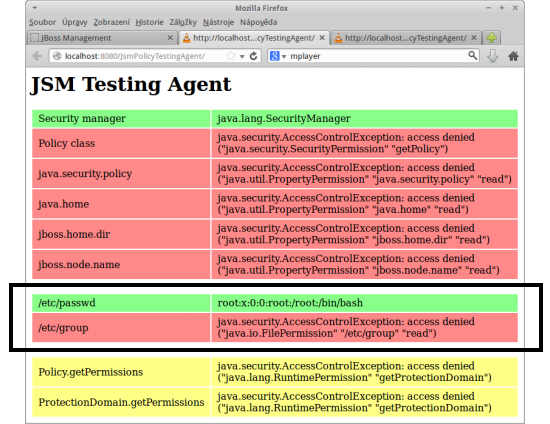
\includegraphics[width=10cm]{fig/test-passwd}
  \caption{Výstup testovací aplikace pro bezpečnostní politiku {\tt passwd-only} -- testovací aplikace může číst obsah souboru {\tt /etc/passwd}, ale ne obsah souboru {\tt /etc/group}}
  \label{testPasswd}
\end{figure}
\begin{figure}[ht]
  \centering
  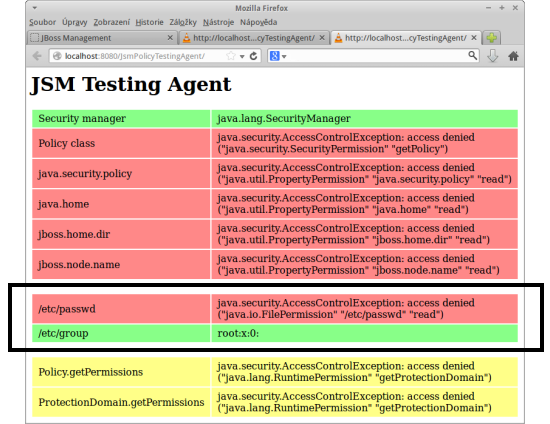
\includegraphics[width=10cm]{fig/test-group}
  \caption{Výstup testovací aplikace pro bezpečnostní politiku {\tt group-only} -- testovací aplikace může číst obsah souboru {\tt /etc/group}, ale ne obsah souboru {\tt /etc/passwd}}
  \label{testGroup}
\end{figure}

%\chapter{Manual}
%\chapter{Konfigrační soubor}
%\chapter{RelaxNG Schéma konfiguračního soboru}
%\chapter{Plakat}

